\section{Fundamentos teóricos}

\subsection{Observaciones solares y esquema de clasificación Zurich--McIntosh}

Las manchas solares corresponden a regiones fotosféricas de menor temperatura relativa, asociadas con concentraciones intensas de campo magnético. Su número, posición y morfología varían a lo largo del ciclo solar, por lo que su registro sistemático permite estudiar tendencias temporales, asimetrías hemisféricas y fases de migración latitudinal \citep{hale1919magneticpolarity,hathaway2015solarcycle,murakozy2022asymmetries}.

La observación solar puede realizarse desde instrumentos espaciales o desde observatorios terrestres. Los primeros ofrecen continuidad y estabilidad radiométrica, mientras que los segundos permiten implementar sistemas académicos accesibles, aunque condicionados por atmósfera, enfoque, estabilidad mecánica y calidad óptica. Por ello, el trabajo adopta una estrategia complementaria entre datos de referencia, reportes NOAA SRS e imágenes capturadas localmente \citep{scherrer2012hmi,bobra2014sharp,noaaSRS,sidcGroundObservations2026}.

\begin{figure}[H]
    \centering
    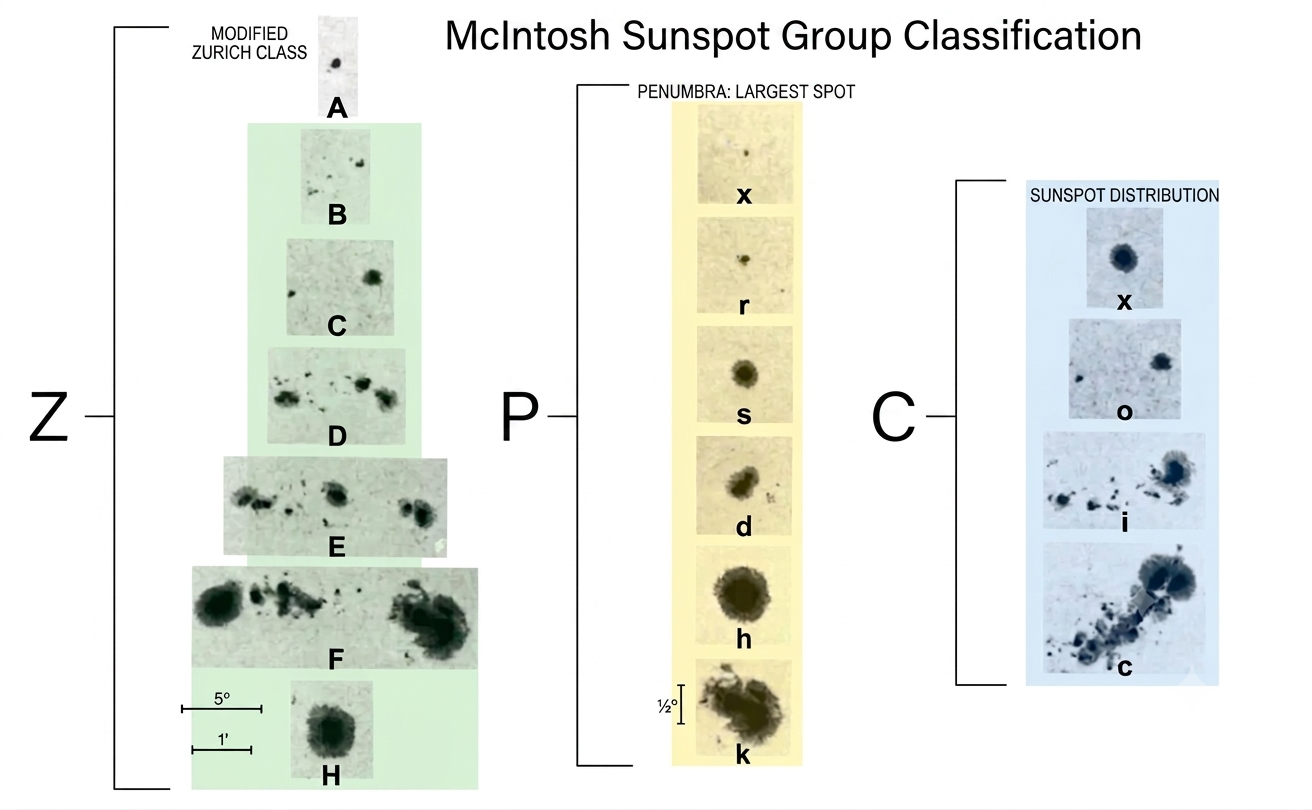
\includegraphics[width=0.7\linewidth]{figures/solar/mcintosh.png}
    \caption{Esquema de la clasificación Zurich--McIntosh utilizada para describir grupos solares. \textbf{Fuente:} Adaptado de criterios observacionales clásicos.}
    \label{fig:resumen-mcintosh}
\end{figure}

La clasificación Zurich--McIntosh describe cada grupo mediante tres componentes: clase evolutiva $Z$, tipo de penumbra $P$ y distribución interna $C$. La etiqueta final puede representarse como
\begin{equation}
    y = (Z,P,C), \qquad y \in \mathcal{Y}_{\mathrm{ZM}},
\end{equation}
donde $\mathcal{Y}_{\mathrm{ZM}}$ contiene únicamente combinaciones morfológicamente válidas. Esta formulación favorece una clasificación jerárquica, más interpretable que una clase plana de combinaciones, porque conserva la relación entre evolución global, estructura penumbral y compactación interna del grupo \citep{mcintosh1990classification,bornmann1994flarerates,watson2009wilson}.

\subsection{Agrupamiento y clasificación de manchas solares}

Los trabajos recientes sobre clasificación automática de regiones activas muestran que el aprendizaje profundo puede reproducir criterios observacionales de Mount Wilson y Zurich--McIntosh, aunque el desempeño depende de la calidad de las etiquetas, del balance entre clases y de la forma en que se incorporan restricciones físicas o taxonómicas \citep{sayez2023sunscc,zhou2023mcintosh,deng2025mcintosh}. En esta tesis se adopta, por ello, una estrategia modular: primero se agrupan y recortan regiones candidatas; luego se clasifican los recortes en los componentes $Z$, $P$ y $C$.

La primera etapa se formula como un problema de detección de objetos. Un detector de la familia YOLO estima cajas delimitadoras $b_i=(x_i,y_i,w_i,h_i)$ para cada grupo solar visible en una imagen de disco completo \citep{ultralyticsYOLO26,robUSET2026,noaaSRS,scherrer2012hmi}.

La segunda etapa recibe los recortes generados por el detector y estima la etiqueta Zurich--McIntosh. En lugar de aprender una única clase plana para cada combinación $ZPC$, el sistema emplea una arquitectura jerárquica basada en ConvNeXtV2 \citep{woo2023convnextv2,mcintosh1990classification}.

\subsection{Modelos predictivos de la actividad solar}

La predicción de la actividad solar anticipar la evolución del ciclo a partir de series históricas como el número de manchas solares, el área activa o la distribución latitudinal de los grupos, la literatura reúne enfoques de precursores físicos, modelos estadísticos de series temporales y métodos de aprendizaje automático o identificación dinámica \citep{pesnell2012predictions,clette2014revisiting,camporeale2019ml}.

Entre los métodos físicos, los precursores basados en campos polares e índices geomagnéticos ofrecen información temprana sobre la amplitud esperada de un ciclo, pero no siempre describen con detalle la evolución mensual del índice de manchas \citep{schatten2005precursor,svalgaard2005polar}. Para complementar esa limitación, la tesis incorpora un bloque PVL--Kalman que suaviza y actualiza recursivamente el número de manchas solares suavizado \citep{kalman1960newapproach,podladchikova2012kalman}.

Sin embargo, una serie escalar no conserva por sí sola la información espacial del ciclo solar. La migración de las bandas activas hacia el ecuador, visible en el diagrama de Spörer, contiene estructura física relevante para interpretar la fase del ciclo y las asimetrías latitudinales \citep{hathaway2015solarcycle,murakozy2022asymmetries}. Por ello, la tesis explora la Descomposición en Modos Dinámicos (DMD) como una línea complementaria de modelado. Cada mes se representa mediante un vector de conteos latitudinales \citep{schmid2010dmd,kutz2016dmd}.

De esta manera, PVL--Kalman aporta una predicción escalar suavizada y DMD agrega una lectura espacio-temporal de la migración latitudinal. La combinación de ambos enfoques no pretende reemplazar los pronósticos operacionales, sino proporcionar contexto físico y visual para el sistema de observación y clasificación desarrollado en la tesis \citep{podladchikova2012kalman,schmid2010dmd,kutz2016dmd}.
